\subsection{Zufälliges generieren von Automaten}
Um Vergleichswerte zu haben, wurde ein Zufallsalgorithmus implementiert, welcher so oft neue Automaten generiert bis einer zufällig der geforderten Lösung entspricht. Der Aufbau des Algorithmus und die Messmethode ist dabei gleich wie bei den zuvor gezeigten. Das heisst, es gibt eine Population welche nach jedem Zyklus neu generiert wird. Dies wird so oft wiederholt, bis ein Zykluslimit erreicht wurde. Gemessen wird wie oft (in Prozent) der Algorithmus eine Lösung findet. In Abbildung \ref{fig:rand_abab} ist ersichtlich, dass dieser Algorithmus bedeutend weniger oft konvergiert als alle von uns untersuchten.

\begin{figure}[h]
  \centering
  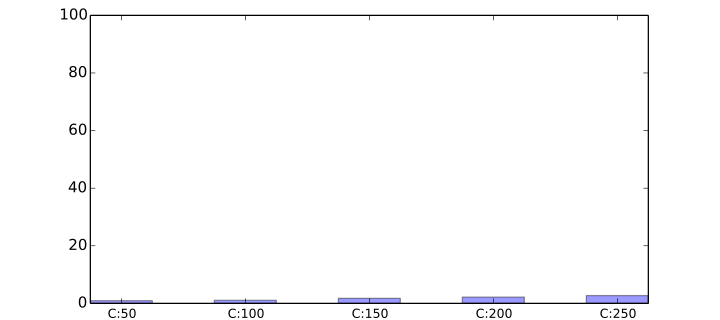
\includegraphics[width=0.80\textwidth]{images/RAND_ABAB_RAND_solved.pdf}
  \caption[Random Algorithmus ABAB Problem]{Random Algorithmus ABAB Problem}
  \label{fig:rand_abab}
\end{figure}